\section{Architecture Overview}

\begin{frame}\frametitle{Architecture Overview}

\begin{enumerate} 
  \item morpheus-graphql-core: The package provides basic language features such as parsing, pretty-printing, and validation of GraphQL queries and schema documents. This package also defines common types and operations used by other packages, such as AST for the GraphQL type system and query language. All other packages depend on this package.

  \item morpheus-graphql-client: The client application enables type-safe client queries. It uses the core package to parse and validate the GraphQL query based on the target server's schema. 
  If the query is valid, it generates the corresponding query and response types using Template Haskell. However, it will throw a compilation error with a   descriptive message on the invalid query.
    
  \item morpheus-graphql-app: this package provides utilities for creating executable GraphQL applications for servers.  Its primary task is to execute the 
  GraphQL document representation parsed by the core package. 
  Therefore it defines internal resolver value interpretations, resolver monads for GraphQL servers, and event action types for GraphQL 
  subscriptions. One can use it to build a schema-first GraphQL server 
  with dynamic typing, where the core package parses 
  the GraphQL document and the app package executes it. 
  That is, the server package is not necessary for this. 
  Although without it, the type-safety is not guaranteed. 
  
  \item morpheus-graphql-subscriptions: This package provides GraphQL subscriptions based on the WebSockets library. 
  It uses the core package and builds a WebSocket server 
  with an \expr{App e m} argument provided by the app package. 
  In other words, it is independent of the server package and 
  accepts any \expr{App e m} derived from an arbitrary server 
  (even from a third-party library). Therefore, it is not relevant to our thesis topic, and we skip the implementation details.

  \item morpheus-graphql: This package depends on the core and app packages and derives \expr{App e m} with native Haskell types by mapping them to GraphQL representations. As a result, the final derived application can be executed by app and subscriptions packages.
  This package also leverages Template Haskell and enables importing type definitions from the GraphQL schema. In particular, the \expr{importGQLDocument} function defines corresponding native Haskell types for each GraphQL type. Users can then provide resolver values for these types, from which the Morpheus compiler derives a server application. 
  This package also provides the function \expr{compileTimeSchemaValidation} for compile-time schema validation, which checks if the API definition represents a valid GraphQL schema.

\end{enumerate}

\end{frame}

\begin{frame}
%!TEX root = ../../main.tex

\begin{figure}
\caption{
    Dependency Graph of the Morpheus GraphQL Packages
    \label{fig:dependency-graph}
    }
\begin{center}
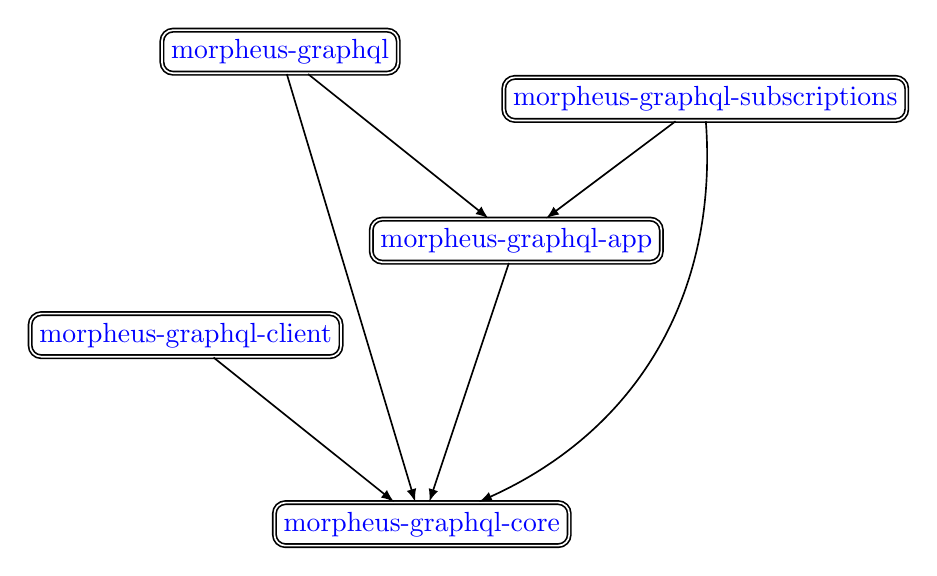
\begin{tikzpicture}[
        scale=.6,
        auto=left,
        -latex ,
        auto ,
        node distance =2 cm and 2cm ,
        % on grid ,
        semithick ,
        package/.style ={ fill=red!20,draw,double,rounded corners ,top color =white ,draw , text=blue , minimum width =1 cm},
    ] 
    \node[package] (core) at (10,0) {morpheus-graphql-core};
    \node[package] (client) at (5,4)  {morpheus-graphql-client};
    \node[package] (app) at (12,6)  {morpheus-graphql-app};
    \node[package] (server) at (7,10)  {morpheus-graphql};
    \node[package] (subs) at (16,9) {morpheus-graphql-subscriptions};
  
    \path (client) edge (core);
    \path (app)  edge (core);
    \path (server)  edge  (core);
    \path (server)  edge  (app);
    \path (subs)  edge  (app);
    \path 
        (subs) 
            edge [bend left =35] 
        (core);  

\end{tikzpicture}
\end{center}
\end{figure}

\end{frame}
